
%%%%%%%%%%%%%%%%%%%%%%%%%%
\chapter{Bayesian Estimation of Seizure Likelihood}
\label{ch:3Bsle}

The recently reported paradigm shift from binary classifications to probabilistic forecasts of seizure risk has been illustrated conceptually in recent works such as \shortcites{karoly2017circadian, baud2018multi}\citet{karoly2017circadian, baud2018multi, baud2020chance}. They discuss the need to consider \emph{pro-ictal} states - states to which we attribute a higher seizure likelihood, that does not necessarily result in a seizure. The likelihood is based on a priori knowledge or assumptions.

In our work, we propose a Bayesian inference based algorithm, namely Bayesian Seizure Likelihood Estimation (BSLE)\footnote{code can be found at \url{https://github.com/noamsgl/msc} under the MIT license.}, and evaluate it on intracranial EEG from canines with epilepsy. It is different than the previously mentioned works by estimating the likelihood in an unsupervised way, dismissing the need for accurate seizure event labels.

%%%%%%%%%%%%%%%%%%%%%%%%%%%%%%%%%%%%%%%%%%%%%%%%%%%%%%%%%%%%%%%%%%%%%%%%%%%%%%%%%%%%%%%%%%%%%%%%%%%%%%%%

\section{Background}
The purpose of this section is to introduce preliminary concepts necessary to understand the probabilistic approach.

% Lower the section header to match the (very) long chapter header
% \renewcommand*\sectionmarkformat{\\ \autodot\thesection\enskip}
%%%%%%%%%%%%%%%%%%%%%%%%%%


% \renewcommand*\sectionmarkformat{\autodot\thesection\enskip}
%%%%%%%%%%%%%%%%%%%%%%%%%%
\subsection{Problem description}
\label{sec:2background:setup}

There is a continuous EEG recording system sampling at $f$ Hz (see figure \ref{fig:c3bsle:caninedb}). We are provided with a dataset $D = \{e_t, a_t\}_{t_0}^{t_m}$. For each time $t$, $e_t \in \mathbb{R}^{c \times f \cdot T}$ is the observed EEG segment with $c$-channels of duration $T$, ending at time $t$. Also, $a_t \in \{0, 1\}$ is a clinically-approved seizure annotation corresponding to the observed interval $[t - T, t]$. The annotation denotes the expert's best judgement as to whether a seizure event began within the corresponding time-window.

The problem at hand is to find a forecaster $f_\tau^*$ with 
predictive qualities of interest. First, a general definition of seizure forecasting is provided. This setup is made more specific in the evaluation section (\ref{sec:c3bsle:results}).

\begin{definition}[seizure forecaster with horizon $\tau$]
    a function of the form $$ \hat{s}_{t+\tau} = f_\tau(e_t, a_{0:t})$$ where $s_{t+\tau}$ is the seizure risk in the interval $[t, t+\tau]$,  $e_t$ is the current EEG observation, $a_{0:t}$ is the past event history, and $\tau$ is the forecast horizon. The horizon parameter $\tau$ can take negative values, to mean detecting seizure events post-observation.
\end{definition}

\begin{figure}[p]
    \centering
    \includegraphics[width=\textwidth]{c3Bsle/Figs/canine/MayoClinic_CanineEpilepsy_print.pdf}
    \Caption{Data collection and required output}{From \citet{coles2013feasibility}. Used with permission of Mayo Foundation for Medical Education and Research, all rights reserved.\vspace{3mm}\\ The Canine-Epilepsy dataset was used for empirical evaluation in this chapter, chosen primarily because it is publicly available and the per-subject recording length is long. The EEG is collected and processed by a forecasting algorithm to produce a seizure risk gauge (bottom).}
    \label{fig:c3bsle:caninedb}
\end{figure}
\clearpage

\subsection{Probabilistic representation of EEG and seizures in time}
\label{sec:c3Bsle:model}

We capture the notion of EEG observations and seizure events by random variables (r.v.s):

\begin{align}
	 e_t \sim E(t) &\in \Omega_E = \mathbb{R}^{c \times N}\\
	 s_t \sim S(t) &\in \Omega_S = \{0, 1\}
\end{align}

where $\Omega_{E}$ ($\Omega_{S}$) is the sample space for the r.v. $E$ (the r.v. $S$). $c$ is the number of EEG-channels, $N$ is the number of samples recorded (\aka segment length) over a duration $T$. We define the event that a seizure began within $[t-T, t]$ as $\{S(t) = 1\}$ (see figure \ref{fig:c3bsle:sample_space}). 

\begin{figure}[!ht]
    \centering
    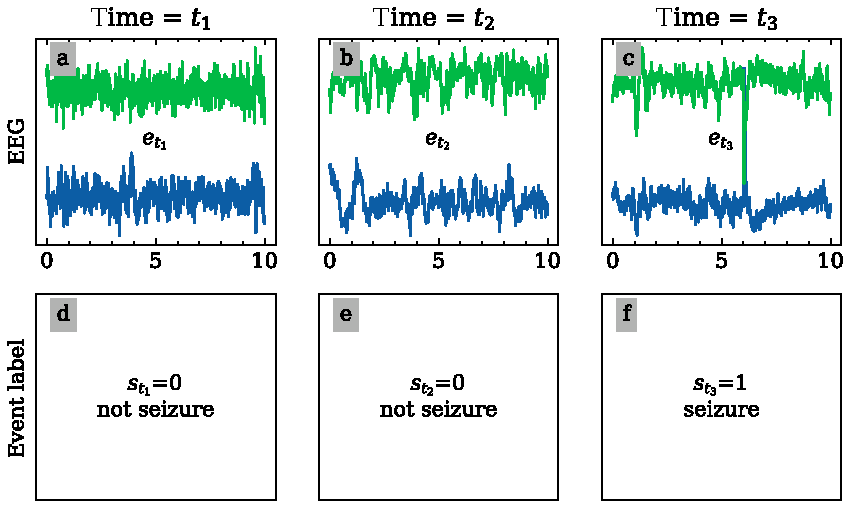
\includegraphics{c3Bsle/Figs/intro/sample_space.pdf}
    \Caption{Sample space $\Omega_E \times \Omega_S$}{In the probabilistic model, EEG segments and seizures are plausible events. For example, a 2-channel 400 $Hz$ EEG segment of length 10 seconds is a realization of the random variable E 
    supported by $\mathbb{R}^{2 \times 400}$. Likewise, the occurrence of a seizure at time $t_i$ is denoted by $s_{t_i} = 1$ as opposed to $s_{t_i} = 0$.}
    \label{fig:c3bsle:sample_space}
\end{figure}



\section{Model specification}
Formally, the proposed model is a multilevel probabilistic model, as shown in figure \ref{fig:c3bsle:bsle_net_intro}. To overcome the curse of dimensionality, first the raw time signal is embedded in a low dimensional manifold. Then, Bayesian inference is applied with custom evidence, prior and likelihood functions to infer the probability $\prob(s_t \mid e_t)$.

% Representing a typical 10-second EEG segment requires about \num{6.4e4} scalar values in it's raw form, thus special care is taken to overcome the curse of dimensionality. 

% partial Bayesian Seizure Annotation Model
\begin{figure}[htbp]

  \tikz{

    % nodes
     \node[obs] (e) {$e_{t}$};%
     \node[latent, above=of e, xshift=1cm] (s) {$s_{t}$}; %
    \node[obs, below=of s, xshift=1cm] (a) {$a_{t}$};%

    % gates

    % edges
     \edge {s} {e, a}

    % plates
    \plate[inner sep=10pt] {plate1} {(e)(a)(s)} {time $t$}; %

    % text
     \node[text width=6cm, anchor=west, right] at (4,1)
     {
       \begin{alignat*}{3}
        e_t & \mid s_t \sim \mathcal{D}_{E \mid S} && \text{ // EEG embeddings conditioned on seizure variable}\\
        a_t & \mid s_t \sim \mathcal{D}_{A \mid S} && \text{ // Annotation conditioned on seizure variable}\\
       \end{alignat*}
     };
   }
 \Caption{Probabilistically Modeling Seizure Occurrence, EEG signal and Annotations across Time}{The nodes represent random variables. The shaded nodes $e$ and $a$ represent the observed variables EEG and Annotations, respectively. The $s$ node represents a latent variable, whose values can be inferred with Bayes' theorem. The }
  \label{fig:c3bsle:bsle_net_intro}
\end{figure}

\subsection{EEG embedding}
\label{sec:c3bsle:embedding}
A Gaussian process (GP) is a mathematical entity often used in Bayesian time series modeling. It allows flexible modeling of smoothness, periodicity and other interpretable signal properties. Existing algorithms which perform posterior inference over the underlying hyperparameters are available \cite{rasmussen2003gaussian, gardner2018gpytorch}. We embed the EEG data in the low-dimensional manifold of GP hyperparameters (see figure \ref{fig:c3bsle:embeddings}). These hyperparameter values are then used to represent the EEG in the following procedures. Technical details of the embedding process are provided in appendix \ref{apx:GPEmbed}.

\begin{figure}[h]
      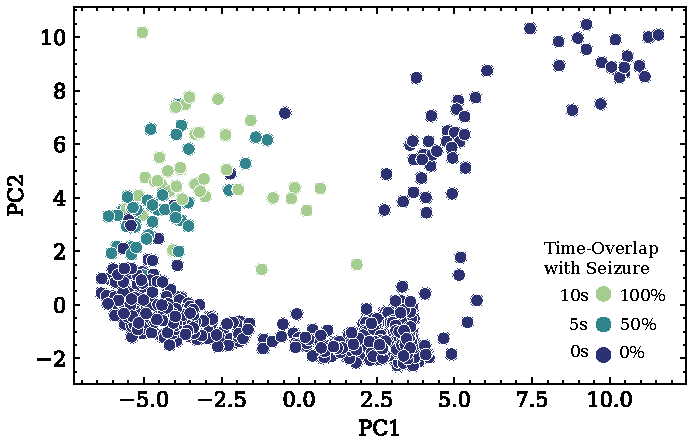
\includegraphics[width=\textwidth]{c3Bsle/Figs/embeddings/embeddings_double.pdf}
      \Caption{EEG embedding in Gaussian process hyperparameter space}{Each point represents a 10-second EEG segment fit with a Gaussian process, and displays the first two principal components of the hyperparameters vector. The color indicates the time of the recording relative to the seizure annotations. The ictal embeddings are found to be distinguishable from the interictal embeddings in the space of GP-hyperparameters.}
      \label{fig:c3bsle:embeddings}
\end{figure}


\subsection{Bayesian estimation}
We wish to construct a model for $\prob[S, E, t]$, and then apply it with Bayes' rule to infer the likelihood of a seizure at time $t$ determined by an EEG recording:

\begin{equation}
\texttt{probability}[\texttt{seizure=}S \mid \texttt{time=}t, \texttt{EEG=}E] \propto \prob[E \mid S, t] \prob[S \mid t]
\end{equation}

It should be evident that this procedure is general in that each component on the right-hand-side can be estimated independently, and then combined via multiplication.

In the case of epilepsy, handling uncertainty in the face of evidence plays a major role, thus naturally appealing to the mathematical machinery termed Bayes' theorem.

We apply Bayes' theorem to estimate the updated likelihood of a seizure after observing an EEG signal:

% \begin{align}
%     \underset{posterior}{\prob(S \mid E)} = \frac{\prob(E \mid S) \prob(S)}{\prob(E)} \propto \underset{likelihood}{\prob(E \mid S)} \cdot \underset{prior}{\prob(S)}
% \end{align}


\begin{align}
    \underset{posterior}{\prob(S \mid E)} = \frac{\underset{likelihood}{\prob(E \mid S)} \underset{prior}{\prob(S)}}{\underset{evidence}{\prob(E)} } 
\end{align}


For bayesian inference, the likelihood, prior and evidence functions need to be defined and approximated. We now derive the mathematical formulations for each of these, which should complete the description of our inference procedure.


\subsubsection{Likelihood Definition}
For a patient with epilepsy, we hypothesize that the anomalies in EEG data are inherently more likely to reflect underlying seizure events, because seizures are rare events. First, we define an unsupervised density-quantile novelty score. Then, we establish the seizure likelihood function by adding a threshold parameter.

\paragraph{Density estimation}
A Gaussian mixture model (GMM) with 4 components and full inter-component covariance matrix is fit to the data in GP-hyperparameter space, to give a density estimation:

\begin{definition}{Density estimation}
    $\hat{p}(e) \approx pdf(E)$
\end{definition}
\label{eq:c3bsle:de}

Mathematical details are provided in appendix \ref{apx:GMM}. See figure \ref{fig:3bsle:de}.

\begin{figure}[hp]
    \centering
    \begin{subfigure}[h]{\floatwidth}
        \showthe\textwidth
          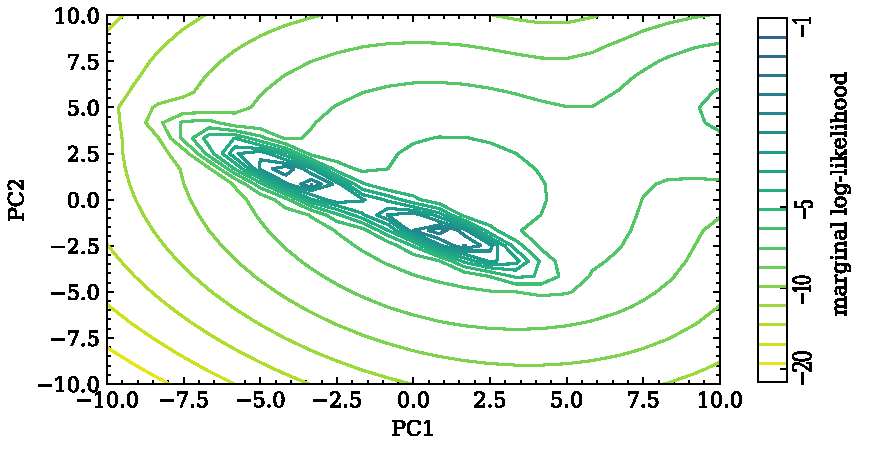
\includegraphics[width=\textwidth]{c3Bsle/Figs/densityestimation/de_pc1_pc2.pdf}
          \caption{First and second principal components}
    \end{subfigure}
  	\begin{subfigure}[h]{\floatwidth}
  	    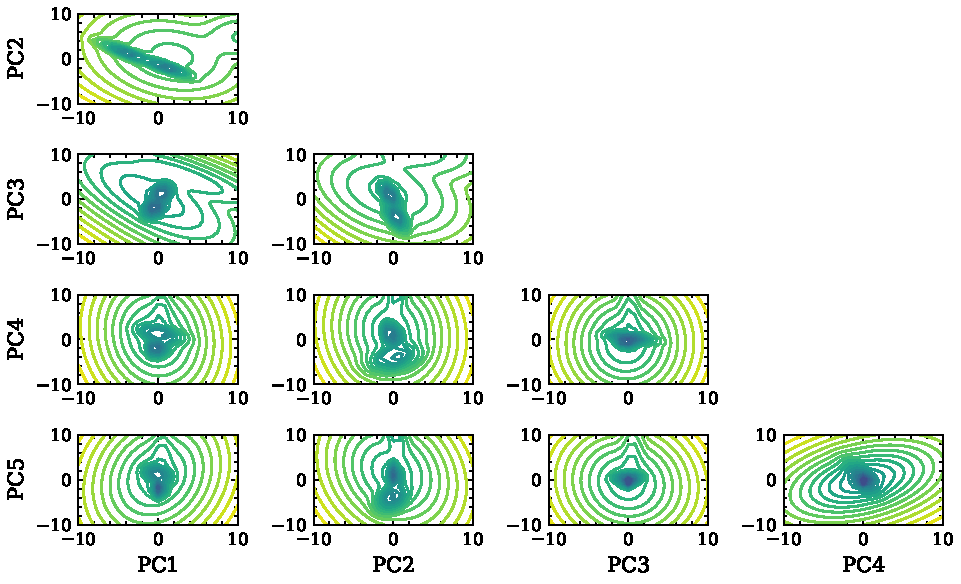
\includegraphics[width=\textwidth]{c3Bsle/Figs/densityestimation/de_pc_pair_plot.pdf}
  	    \caption{Pair plots for the first five principal components}
  	\end{subfigure}
    \Caption{Contour plots for multidimensional density estimation}{An estimator $\hat{p}(e_t)$ is computed using a GMM with 4 components fit to the first 5 principal components of the data as represented by GP hyperparameters. The contour plot of $\log \hat{p}(e_t)$ is shown for every pair of principal components by marginalizing 
    over the remaining axes. The regions with lower likelihood are more likely to be classified as seizures.}
    \label{fig:3bsle:de}
\end{figure}



\paragraph{Density quantile approach to Novelty Scores}

A Monte Carlo technique, namely the Density Quantile Approach, is used to obtain information about the probability coverage of a given region of the sample space. Given a new sample $e$, the novelty score is the quantile (also known as a $p_{value}$) of $\hat{p}(e)$ relative to the random variable $E$, as approximated by a sample dataset $D$. This calculation has been shown to converge tractably to the probability density function quantile as the sample size grows \cite{hyndman1996computing}. 

\begin{definition}{Novelty Score}
    \begin{equation}
    \label{eq:c3bsle:novelty_score}
    \mathcal{Z}(e^{new}) = \frac{\left|\{ e_i \mid \hat{p}(e^{new}) \le \hat{p}(e_i) \} \right|}{|\{ e_i\} |}
    \end{equation}
\end{definition}

The essence of the novelty score $\mathcal{Z}(e^{new})$ is that it maps data samples to the interval $[0, 1]$, such that more anomalous samples (i.e. samples from less dense regions) are given larger values.

In accordance with our rarity of seizures hypothesis, a new normal (nonseizure) EEG observation $e^{new}$ will be relatively similar to previously seen observations in $\{ e_i \}$, leading to a low novelty score. Conversely, for abnormal (seizure) data, the data will be relatively dissimilar, leading to a high novelty score.

In order to utilize this hypothesis in the BSLE likelihood function, we flip the sign of the $S$ parameter to $\neg S$ meaning not a seizure, thus modeling $\prob(E \mid \neg S)$ directly.

\paragraph{Partitioning with a threshold $\alpha$}
A new threshold parameter $\alpha$ is introduced to guide the BSLE likelihood function $P(E \mid \neg S ; \alpha)$. Using the density estimator $\hat{p}(e)$, we partition the GP-hyperparameter sample space $\Omega_{GP}$ into a low density region and a high-density region, and treat each region differently. The threshold parameter $\alpha$ affects the location of the region split.

\begin{definition}[$\alpha$-Highest Density Region]
    Let $f(x)$ be the density function of a random variable $X$. Then the $100(1-\alpha)\%$ HDR is the subset $R(f_\alpha)$ of the sample space of $X$ such that
    $$R(f_\alpha) = \{ x : f(x) \ge f_\alpha \}$$
    where $f_\alpha$ is the largest constant such that $\prob(X \in R(f_\alpha)) \ge 1-\alpha$.
\end{definition}
 
\begin{definition}[BSLE likelihood]

% \prob\!\left(E \middle\vert \neg S\right) 
\begin{equation}
\label{eq:c3bsle:likelihood}
\prob(e^{new} \mid \neg S ; \alpha) = \begin{cases}
\mathcal{Z}(e^{new}) &\text{if $e^{new} \in HDR_\alpha$}\\
0 &\text{if $e^{new} \notin HDR_\alpha$}
\end{cases}
\end{equation}

Intuitively, the $\alpha$ parameter determines the interplay between auto-rejection of a sample and estimation of its seizure likelihood. 
\end{definition}



\subsubsection{Evidence Definition}
\begin{definition}[BSLE Evidence]
    \begin{equation}
    \label{eq:c3bsle:evidence}
    \prob(E) = \prob(\{pdf(e) \leq pdf(E)\})
    \end{equation}
\end{definition}


\subsubsection{Prior definition}
The prior function is where the Bayesian modeler induces intentional bias into the inference process. We define and compare two priors, to show that our model is general in this respect.

\paragraph{Weakly supervised cyclical prior}
This prior encourages forecasters to inhibit a circadian - twenty four hour long - cyclical preference. We construct mathematically the cyclical prior as a linear mixture of 24 circular Gaussian distribution kernels, as in \cite{karoly2017circadian}.

% circular Gaussian distribution definition
\begin{definition}[Circular Gaussian Distribution]
    % $$ \hat{y}_{t+\tau} = f(e_{t-k:t}, a_{0:t})$$
    \begin{align}
    f(x | \mu, \kappa ; \omega) = \frac{\exp (\kappa \cos (\omega (x - \mu)))}{2 \pi I_0(\kappa)}
    \label{eq:2background:vm_density}
\end{align}

In this work, we set $\omega \gets \frac{2\pi}{24}$ to scale the period to 24-hours, and drop it from the notation for brevity in the following text.

% \begin{figure}
%     \centering
%     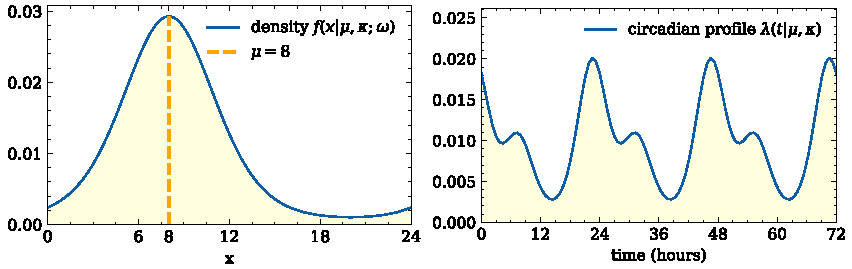
\includegraphics{c3Bsle/Figs/model/vm_and_circadian_profile.pdf}
%     \caption{Caption}
%     \label{fig:my_label}
% \end{figure}
\label{def:circ_gaussian}
\end{definition}


\begin{figure}[h]
    \centering
    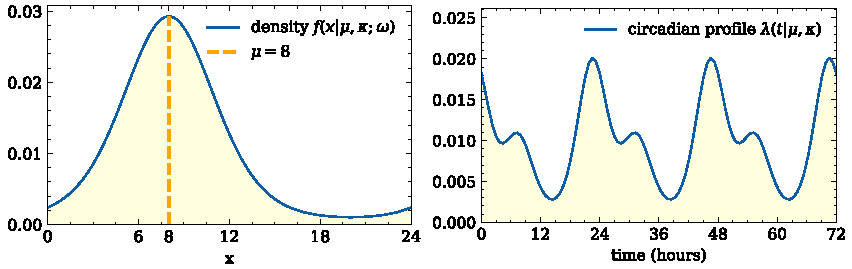
\includegraphics{c3Bsle/Figs/model/vm_and_circadian_profile.pdf}
    \Caption{Circular Gaussian (von Mises) distribution and circadian profile}{
The circular Gaussian distribution is similar to a bell-shaped normal distribution on a circle (left).\\A mixture of von Mises distributions represents the cyclical seizure base-rate behavior, termed \emph{circadian profile} (right).}
    \label{fig:c3bsle:vm}
\end{figure}

% uniform prior definition
\begin{definition}[Circadian prior]
    \begin{equation}
    \label{eq:c3bsle:cyclical_prior}
    \prob(S_t) = \frac{1}{K}\sum_{i=0}^{23} f(t \mid i, k)
    \end{equation}
    where $K$ is a normalizing constant evaluated numerically (\texttt{np.trapz}).
\end{definition}

\begin{figure}[h]
    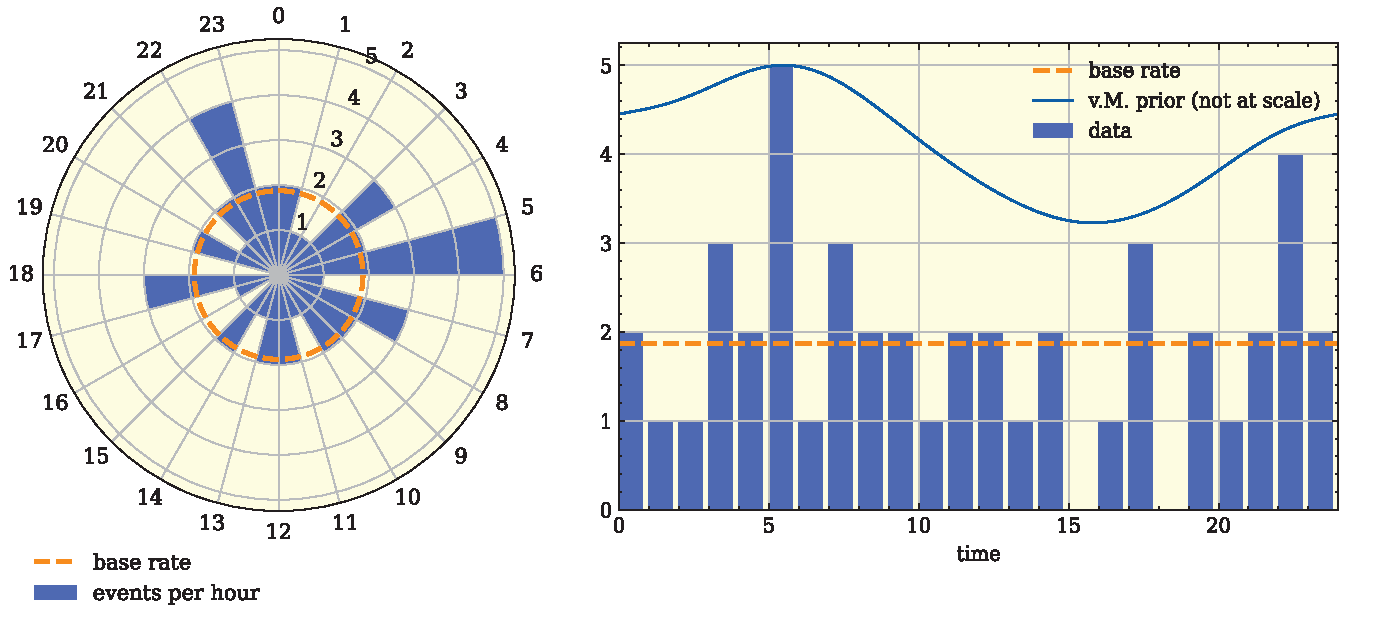
\includegraphics[width=\textwidth]{c3Bsle/Figs/prior/vm_prior_histogram.pdf}
    \Caption{Circadian Seizure Histogram and Circadian Profile}{The 45 seizure events of canine \texttt{I004\_A0003\_D001} from 465 days are binned by hour-of-the-day into a polar histogram (left). A von Mises mixture density function, with kernel weights given by the circadian histogram, is plotted (right).}
    \label{fig:c3bsle:circadian_hist_vm}
\end{figure}

% uniform prior definition
\begin{definition}[Uniform prior]
The uniform prior takes a constant value for all time points: 
    \begin{equation}
    \label{eq:c3bsle:uniform_prior}
    \prob(S_t) = \lambda_0 \cdot T
    \end{equation}
    where $\lambda_0$ is a constant seizure rate, and $T$ is the observation duration.
    Without loss of generality, we set $\lambda_0 = \frac{1}{10 \text{ day}}, T = 10 \text{ sec}$.
\end{definition}
This prior issues equal seizure plausibility to all time points, nullifying the time covariate's effect on the seizure likelihood estimation.

Now, using the fact that $\prob(S) + \prob(\neg S) = 1$, and having observed an EEG recording $E$, the a posteriori estimate for the likelihood of a seizure is given by:

\begin{equation}
\label{eq:c3bsle:posterior}
    \underset{{\substack{\text{probability of seizure}\\\text{given EEG}}}}{\prob(S \mid E)} = 1 - \frac{\prob(\neg S) \prob(E \mid \neg S)}{\prob (E)}.
\end{equation}

which completes the description of the BSLE algorithm.

\clearpage
\section{Empirical results}
\label{sec:c3bsle:results}
The previous subsection described the calculations of the likelihood, priors and evidence functions. We also discussed embedding EEG recordings to the space of Gaussian process (GP) hyperparameters. We now show the results of applying these functions to the embedded recordings, as measured by the receiver operating characteristic curves with respect to the provided annotations.

\subsection{Data}
In this chapter we use the Canine-Epilepsy Dataset. The dataset was curated by \citet{davis2011novel} and made available for the \citet{kaggle2014contests} seizure detection and prediction contests. A canine with natural epilepsy was monitored continuously for 475 days. The monitoring system, consisting of 16-electrode EEG sensors, was implanted in the brain, digitally sampling at the rate of 400 Hz (see figure \ref{fig:c3bsle:caninedb}). Also, 45 seizures were annotated in the dataset following validation by expert visual review of iEEG data and video recordings. The annotations are given as a sequence of timestamps which mark the start of each observed seizure event.


\subsubsection{Train-validation split}
We split the whole timeline into an early training set and a later validation set. The training set consists of 3000 samples of EEG, drawn uniformly from the first 200 days of recording. The validation set consists of another 3000 samples, drawn uniformly from day 200 to day 475. For validation purposes only, the 28 annotated seizure recordings were added to the validation set. 


\subsubsection{Pseudo-prospective study}
First, the training dataset is provided to the BSLE estimator in the \texttt{fit(eeg, prior\_events)} method. If \texttt{prior\_events is None}, the model selects the uniform prior (equation \ref{eq:c3bsle:uniform_prior}). Otherwise, a list of seizure timestamps from the validation phase is given, and the model selects the circadian prior (equation \ref{eq:c3bsle:cyclical_prior}) with kernel weights proportional to the circadian histogram (figure \ref{fig:c3bsle:circadian_hist_vm}). The model then calculates the likelihood function and evidence as given by \cref{eq:c3bsle:likelihood,eq:c3bsle:evidence}.

Only after the \texttt{fit(...)} procedure completes, we call \texttt{predict\_proba(eeg, samples\_times)} for the validation phase, which predicts the probability of a seizure, conditioned on the EEG signal, $\prob(s_t \mid e_t)$ for each sample $e_t$, as given by \cref{eq:c3bsle:posterior}. This separation of concerns ensures simulating a real-time setting in which the  'offline' calibration phase is followed by an 'online' detection mode.

\begin{figure}[hp]
    \centering
    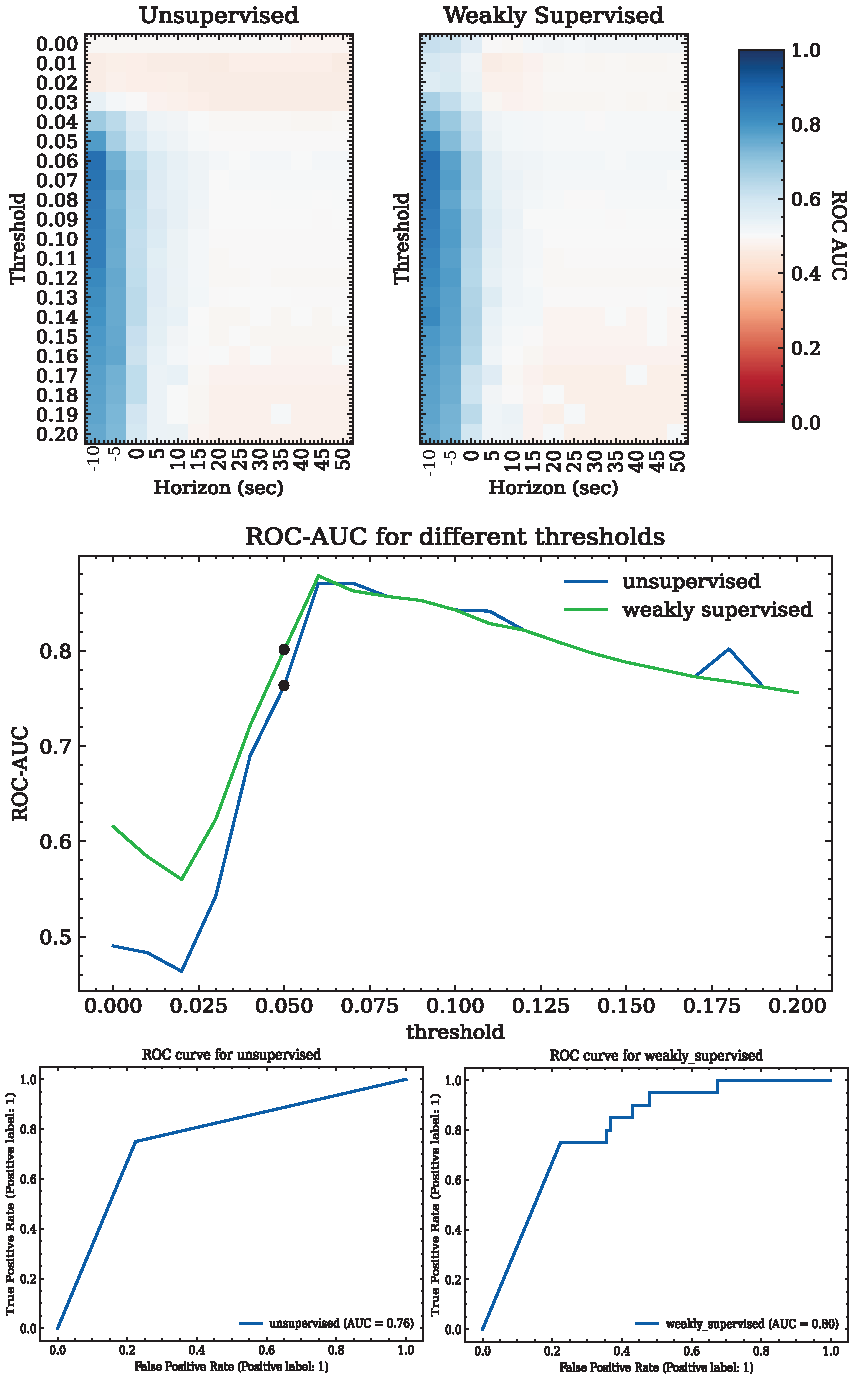
\includegraphics[width=\floatwidth]{c3Bsle/Figs/bsle/roc_grid.pdf}
    \Caption{Empirical results}{AUC-ROC scores smoothly distributed in the hyper-parameter space of both the unsupervised and weakly-supervised models, showing a low risk of overfitting (top row). The ROC-AUC of the weakly supervised model is usually higher than the unsupervised model (middle). An ROC curve is shown for each model when the likelihood threshold parameter is set to $\alpha=0.05$ (bottom).}
    \label{fig:c3bsle:roc_grid}
\end{figure}


% \subsection{Methods for evaluating forecast skill}
% \NS[inline]{write about probabilistic forecast skill evaluation methods}


% \section{Configuring seizure alerts}

% Based on the posterior class probability $\prob(S \mid E, t)$, we will configure warning alerts.
% \NS[inline]{determine method to configure alerts (business decision)}


% \subsection{Bayesian model checking}
% \NS[inline]{write about Bayesian model checking}

% \subsubsection{Prior}

% \subsubsection{Seizure Likelihood Estimation}

% \subsubsection{Model validation}
% \subsubsection{Linear probing}
% % https://arxiv.org/pdf/1610.01644.pdf
% % https://arxiv.org/pdf/2002.05709.pdf
% % https://www.youtube.com/watch?v=HJn-OTNLnoE

% By fitting the SVM to a training set and scoring the predictive accuracy on a hold-out test set, we can quantify the linear separability of the dataset. This is used as a proxy for representation quality.


% In order to further demonstrate the distinguishability between the interictal and ictal states, we show in figure \ref{fig:5results:svm} that a linear-kernel SVM fit to the training set achieves 0.91 AUC on the test set in the single-channel case. The double-channel case scores higher.

% \begin{figure}[htb]
    \centering
    \begin{subfigure}[b]{0.5\floatwidth}
        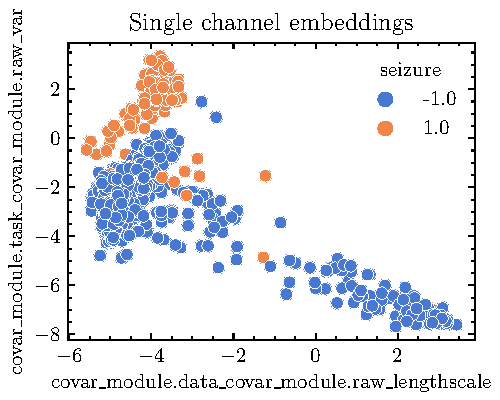
\includegraphics[width=\textwidth]{5Results/figs/svm/svm.pdf}
        \caption{decision boundary}
    \end{subfigure}
    \hfill    
    \begin{subfigure}[b]{0.5\floatwidth}
        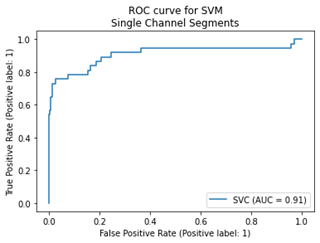
\includegraphics[width=\textwidth]{5Results/figs/svm/svm_roc.png}
        \caption{ROC curve}
    \end{subfigure}
    \hfill
    \Caption{Separability in the parameter space}{
	A support vector machine achieves 0.91 AUC-ROC on a held-out test set for single-channel segments.
	\protect \NS[inline]{remake seperability test figures}
    }
    \label{fig:5results:svm}
\end{figure}



% \subsection{AUC ROC, AUC PR}
% \begin{figure}[htbp]
  \centering
  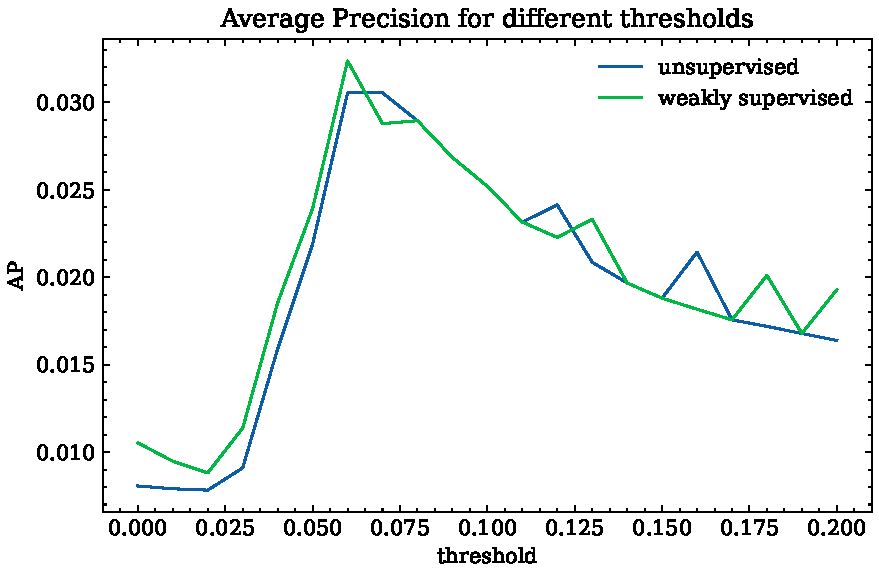
\includegraphics{5Results/figs/bsle/average_precision_score_for_thresholds.pdf}
  \caption{Average Precision scores (higher is better)}
\end{figure}
\begin{figure}[htbp]
  \centering
  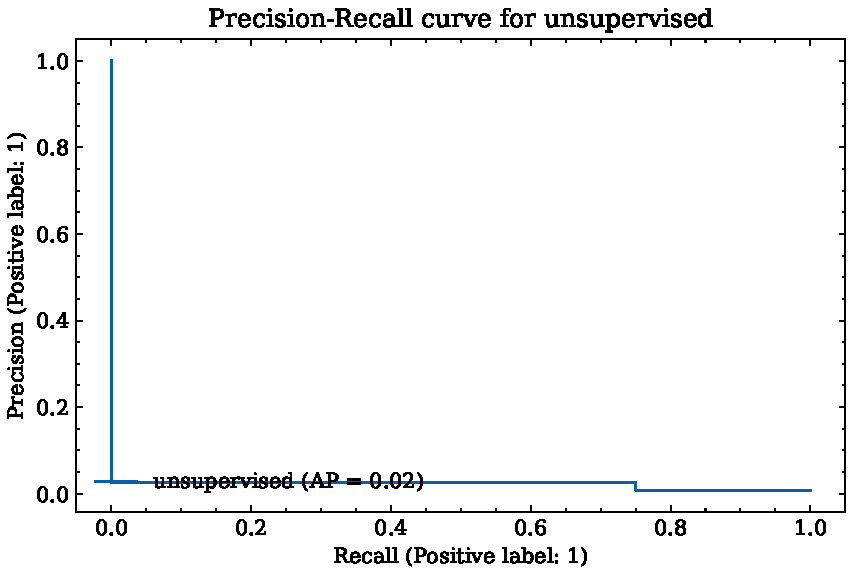
\includegraphics{5Results/figs/bsle/pr_auc_unsupervised.pdf}
  \caption{AP for unsupervised}
\end{figure}
\begin{figure}[htbp]
  \centering
  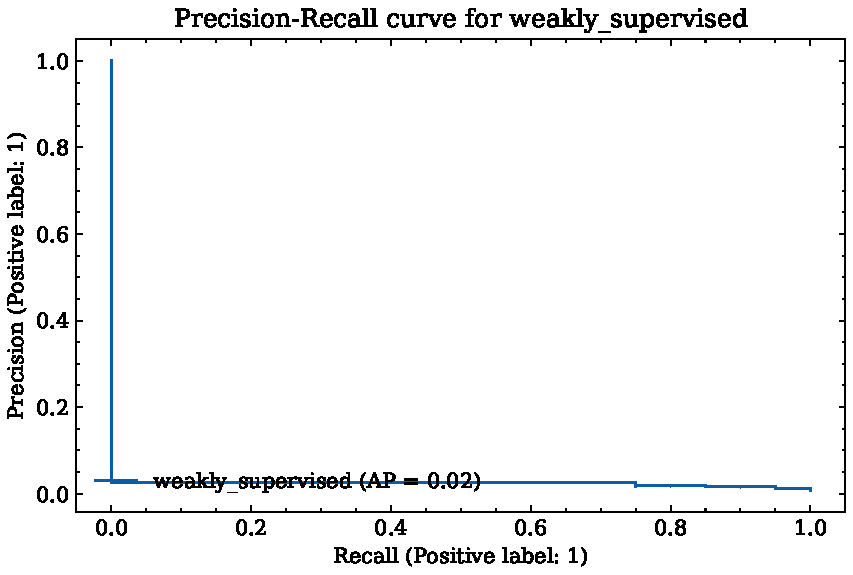
\includegraphics{5Results/figs/bsle/pr_auc_weakly_supervised.pdf}
  \caption{AP for weakly supervised (higher is better)}
\end{figure}
\begin{figure}[htbp]
  \centering
  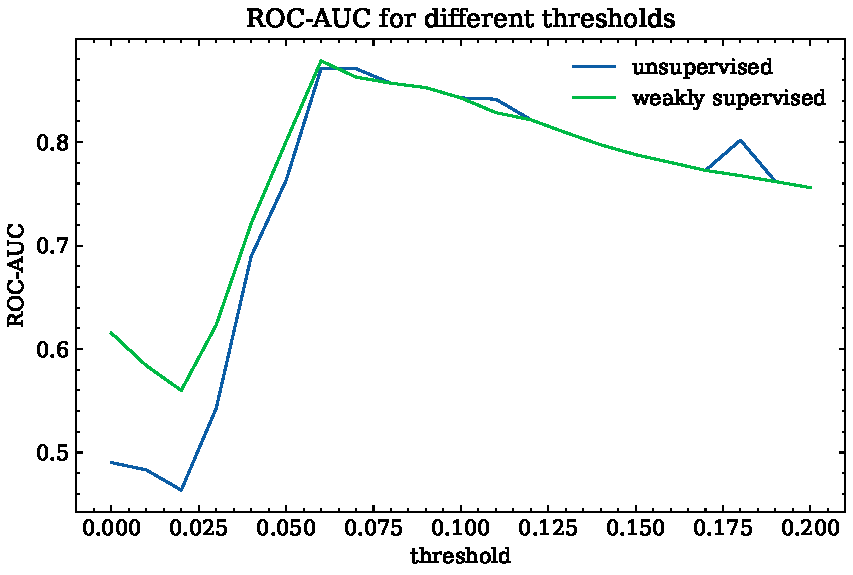
\includegraphics{5Results/figs/bsle/roc_auc_score_for_thresholds.pdf}
  \caption{ROC-AUC scores (higher is better)}
\end{figure}
\begin{figure}[htbp]
  \centering
  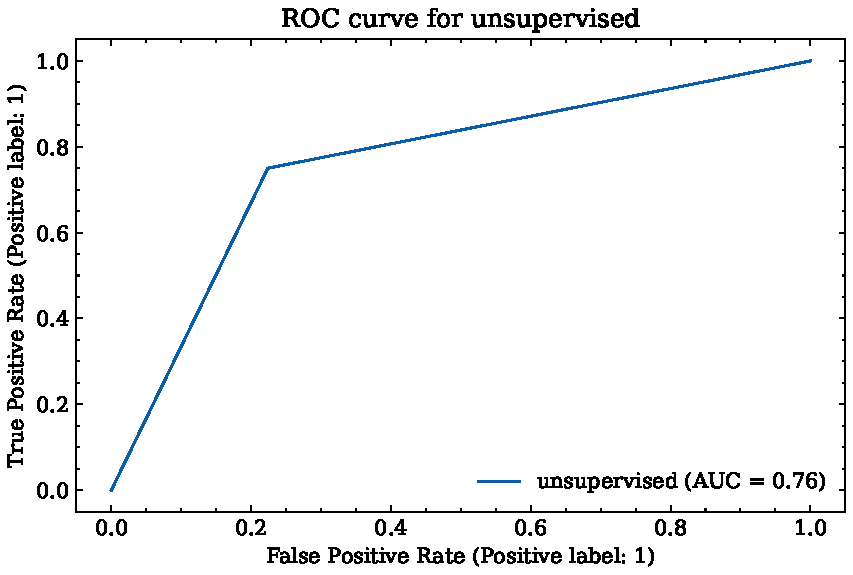
\includegraphics{5Results/figs/bsle/roc_auc_unsupervised.pdf}
  \caption{ROC for unsupervised}
\end{figure}
\begin{figure}[htbp]
  \centering
  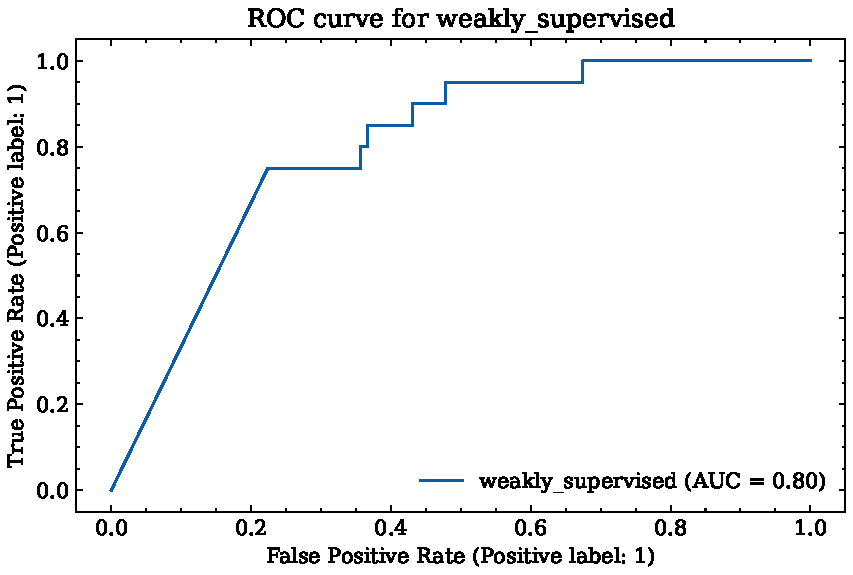
\includegraphics{5Results/figs/bsle/roc_auc_weakly_supervised.pdf}
  \caption{ROC for weakly supervised
  \NS[inline]{check which threshold made the roc curve fig and write it}
  }
\end{figure}
\begin{figure}[htbp]
\centering
  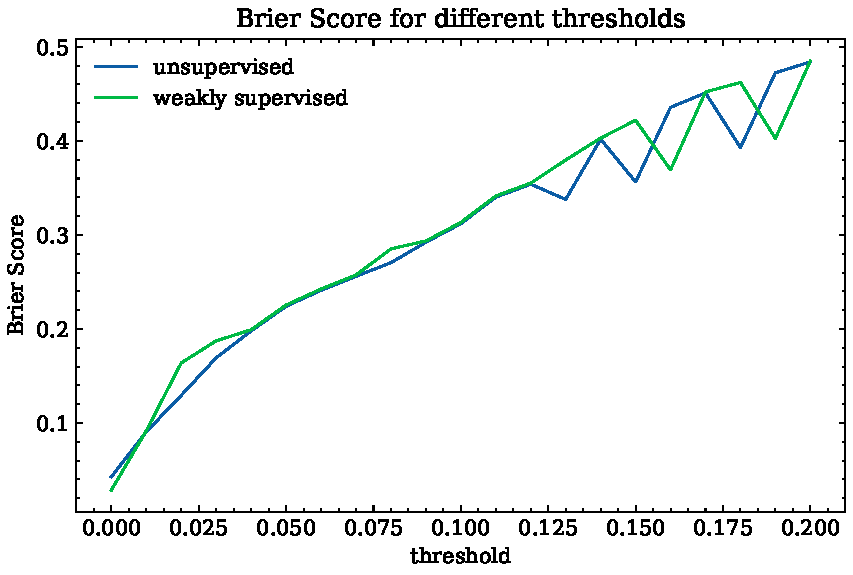
\includegraphics{5Results/figs/bsle/brier_score_for_thresholds.pdf}
  \caption{Brier scores (lower is better)}
\end{figure}
% \begin{figure}[htbp]
% \centering
%   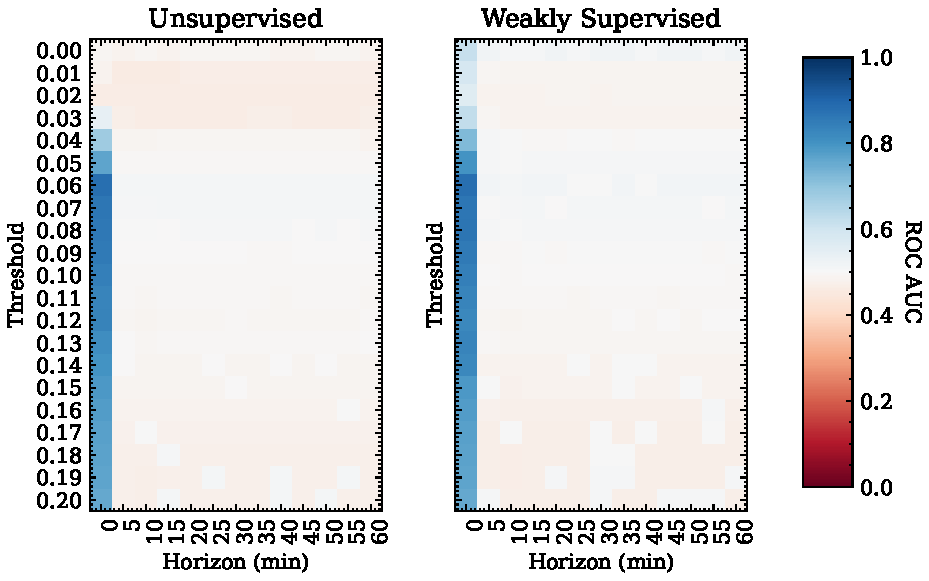
\includegraphics{5Results/figs/bsle/auc_roc_scores_for_thresholds_and_horizons_min.pdf}
%   \caption{AUC-ROC Heatmap for minutes time scale}
% \end{figure}
\begin{figure}[htbp]
\centering
  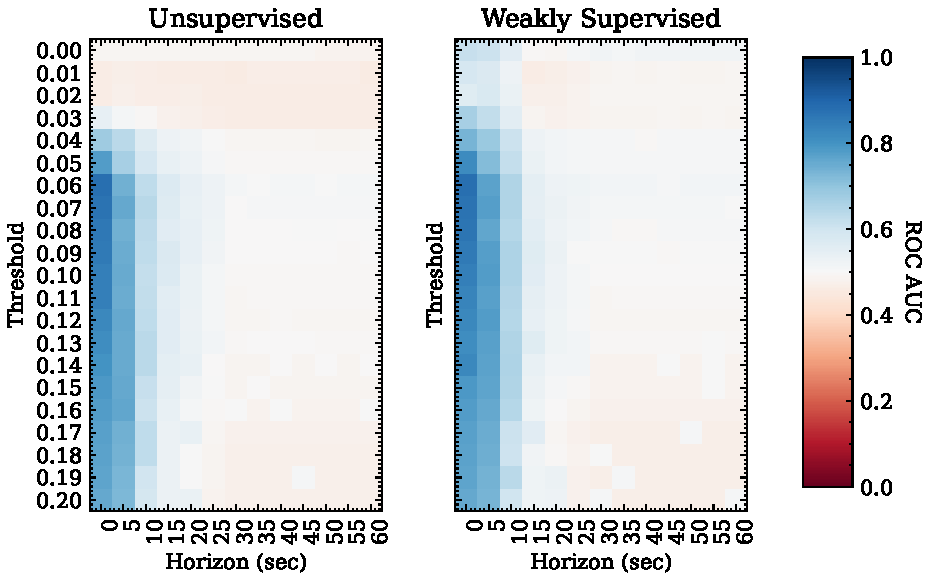
\includegraphics{5Results/figs/bsle/auc_roc_scores_for_thresholds_and_horizons_sec.pdf}
  \caption{AUC-ROC Heatmap for seconds time scale}
\end{figure}
% \Caption{Embedding of EEG}{}
% \label{fig:5results:bsle}


